\chapter{Quantum computational chemistry} \label{Quantum computational chemistry}

\section{Motivation}
Simulating an atomic system is quite a difficult task. In order to understand the full structure and the dynamics of such system, in the non-relativistic approximation, one has to solve the Schrödinger equation
\begin{equation}
    i\hbar\frac{\partial |\Psi\rangle}{\partial t} = H|\Psi\rangle,
\end{equation}
which is also referred to as the time-dependent Schrödinger equation (TDSE). \\
If the Hamiltonian $H$ does not depend on time $t$ the equation can be written as
\begin{equation}
    H |\Psi\rangle = E |\Psi\rangle,
\end{equation}
which is referred to as the time-independent Schrödinger equation (TISE).
This eigenvalue problem leads to find the eigenvectors $\ket{\Psi}$ and the eigenvalues $E$ of the Hamiltonian $H$, which represent the wave function and the energy levels of the system. \\
In this approximation we can also describe the time evolution of the wave function with a unitary operator $U$ in the form of
\begin{equation}\begin{split}
U(t_0,t) |\Psi(t_0)\rangle = e^{-\frac{i}{\hbar}H (t-t_0)} |\Psi(t_0)\rangle = |\Psi(t)\rangle.
\end{split}\end{equation}
This way each eigenvector evolves in time through the action of the operator corresponding to its own eigenvalue. \\
Unfortunately the TISE can be exactly solved only for the hydrogen atom. The solution leads to the wave function states, also called atomic orbitals, shown in Figure \ref{Atomic orbitals}; they are composed of Laguerre polynomials, for the radial variable, and spherical harmonic functions, for the polar and azimuth variables. This result can also be synthesized by using three quantum numbers $(n, l, m)$, called respectively principal, azimuthal and magnetic quantum numbers, to account for the wave functions and the corresponding energy levels. This way the ground state of such atom can be represented by the triplet $(1,0,0)$ or by the symbolic writing $1s$.
\begin{figure}[ht]
  \centering
  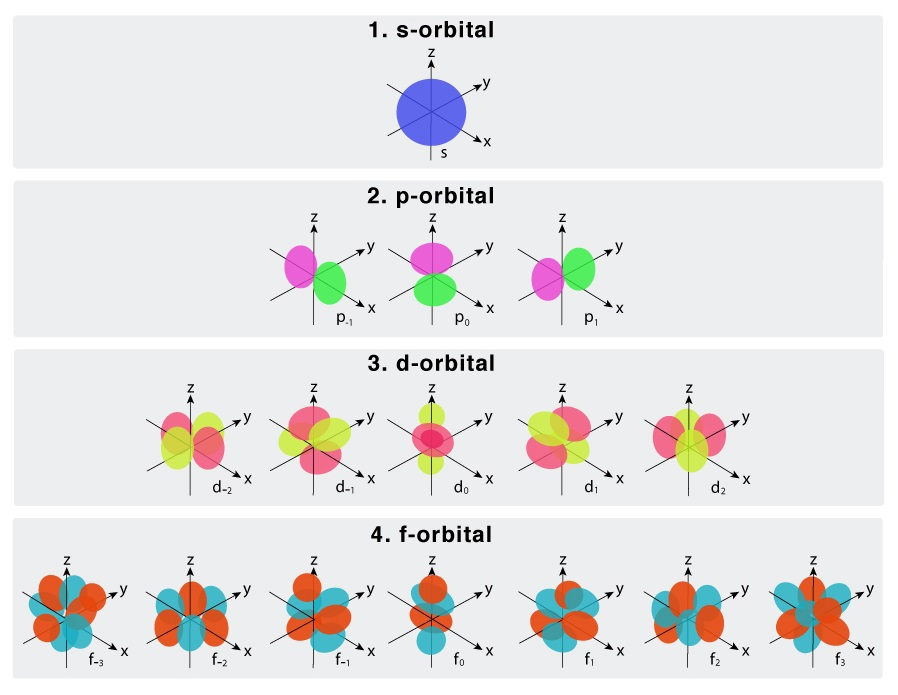
\includegraphics[width=0.7\textwidth]{figures/Atomic orbitals.jpg}
  \caption{Exact atomic orbitals for the hydrogen (H) atom.} \label{Atomic orbitals}
\end{figure} \\
For bigger systems the complexity grows, the terms in the Hamiltonian operator adds up and new terms of interaction appears. The latter, especially, grows combinatorially with the number of electrons and nuclei. \\
The Hamiltonian for a generic multi-electron system can be written as
\begin{equation}\begin{split}
H = -\sum_{i} \frac{\hbar^2}{2m_e}\nabla^2_i
    -\sum_{i} \frac{\hbar^2}{2M_I}\nabla^2_I
    -\sum_{i,I} \frac{e^2}{4\pi\epsilon_0} \frac{Z_I}{r_{iI}} \\
    +\frac12 \sum_{i \neq j} \frac{e^2}{4\pi\epsilon_0} \frac{1}{r_{ij}}
    +\frac12 \sum_{I \neq J} \frac{e^2}{4\pi\epsilon_0} \frac{Z_I Z_J}{r_{IJ}},
\end{split}\end{equation}
with $i,j$ and $I,J$ indicating respectively the electrons and the nuclei. \\
No analytical solution exists for this type of equations. One can use approximations to solve easier versions of these problems, but the amount of calculation needed grows rapidly. This is why, with the advent of digital computers, in the 1950s, a new field of research was born: computational chemistry. \\
\\
The aim is to simulate chemical compounds and materials that are difficult to study from a theoretical point of view, which, as we have seen, are the vast majority, but also to study those systems that are not available to be studied in laboratory or those that need specific and difficult to obtain experimental conditions. Another important use is to employ simulation as a complement to experiments, both to help explain and interpret certain phenomena, for example why a material show a certain property in a certain condition, and to make predictions, that is, one can compare the result of the simulation with the result of the experiment to show if the predictive model used is correct \cite{Szabo1996Jul, Cramer2004Sep}. \\
From this argument, a simple scheme that one can follow to simulate an atomic system is:
\begin{enumerate}
  \item \textbf{Compute the solution for the TDSE or the TISE, with the use of approximations} \\
  A typical approximation is the Born-Oppenheimer approximation, i.e. considering the large difference between the electron mass and the masses of atomic nuclei and correspondingly the time scales of their motion, we can express the total wave function of the system as the product of an electronic wave function and a nuclear wave function, the latter is sometimes called vibrational or rotational.
  \begin{equation}
      |\Psi_{total}\rangle = |\Psi_{electronic}\rangle |\Psi_{nuclear}\rangle.
  \end{equation}
  This enables a separation of the Hamiltonian operator into electronic and nuclear terms. In the electronic Hamiltonian the electron–nucleus interactions are simplified, but not removed, i.e. the nuclei are considered stationary and the electrons "feel" the Coulomb interaction. We also use natural units to simplify the numeric constants,
  \begin{equation}\begin{split}
     H_e = -\frac12\sum_{i} \nabla^2_i
              -\sum_{i,I} \frac{Z_I}{r_{iI}}
              +\frac12 \sum_{i \neq j} \frac{1}{r_{ij}},
  \label{eq:electronic hamiltonian}
  \end{split}\end{equation}
  thus giving us the electronic TISE,
  \begin{equation}
    H_e |\Psi_e\rangle = E_e |\Psi_e\rangle.
  \label{eq:electronic TISE}
  \end{equation}
  By numerically solving the equation (\ref{eq:electronic TISE}) iteratively, changing the position of the nuclei $\textbf{R}$ at every step, we obtain the electronic energy $E_e$ as a function of $\textbf{R}$, this is the potential energy surface (PES). This is often referred to as the 'electronic structure problem'.
  
  \begin{figure}[ht]
  \centering
  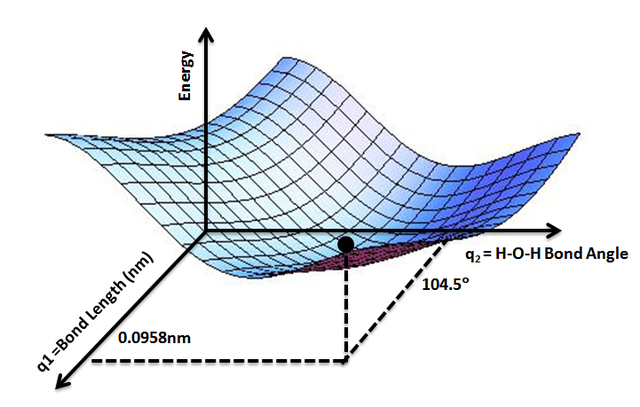
\includegraphics[width=0.65\textwidth]{figures/Potential_Energy_Surface_for_Water.png}
  \caption{Potential energy surface for the water (H$_2$O) molecule.}
  \end{figure}
  
  In principle we can derive the molecular dynamics by computing the unitary evolution of the system, this is referred to as 'ab initio molecular dynamics' (AIMD), since it relies only on fundamental laws of quantum mechanics. In order to obtain the dynamics we need to solve the nuclear TISE, compute the excited states, also called virtual states, of the compounds and the corresponding energy levels. This is because interactions happen between wave functions that are not localized in space, thus multiple eigenstates have to be considered at the same time, this is also called superposition. \\
  In this thesis we will not focus on the problem of molecular dynamics and solutions for the TDSE, but only on the equilibrium phase and the TISE, although it is still a wide and open field of research and there are many methods to solve it, both using digital computers and quantum computers (Ehrenfest method, Born-Oppenheimer molecular dynamics, Car-Parrinello method, quantum phase estimation, Zalka method, to name a few \cite{Poirier2020}).
  
  \item \textbf{From the eigenvectors and the eigenvalues of the TDSE and the TISE compute the chemical properties of the systems} \\
  At the heart of any chemical process there is its mechanism, the elucidation of which requires the identification of all relevant stable intermediates and transition states and the calculation of their properties. The latter allow for experimental verification, whereas energies associated with these structures provide access to thermodynamic stability and kinetic accessibility. In general, a multitude of charge and spin states need to be explicitly calculated in search for the relevant ones that make the whole chemical process viable. \\
  First of all we can study a single compound. From the PES we can find the configurations that lead to the stable structures, i.e. the minima of the multidimensional surface, this procedure is also called 'geometry optimization'. We can also find the optical properties, i.e. study the interaction of the compound with electromagnetic fields. \\
  Second, we can model chemical reactions. We can find the reaction rates and the transition states, i.e. reaction intermediates, which cannot be observed in a laboratory experiment, thus reconstructing the entire path of the reaction. \\
  Moving on to materials, simulation allow us to study thermodynamic and magnetic properties of complex systems, such as cold atomic gases, spin glasses and the Fermi-Hubbard model.
  
  \item \textbf{Apply these methods to bigger and more complex systems} \\
  With simulation we can study both long chains of reactions, e.g. photosynthesis mechanism, which involve many interactions, and individual systems with a big number of highly-correlated particles, e.g. superconducting materials and catalysts. \\
  Some examples of applications are \cite{Bauer2020Nov}:
  \begin{itemize}
      \item \textbf{The chemistry of enzyme active sites} \\
      These can involve multiple coupled transition metals, which present some of the most complicated quantum chemistry problems in the biological world. Combined theoretical and experimental studies have proven successful in unravelling many structural and electronic features of these systems, however, a detailed understanding of the interplay between spin-coupling and delocalization between metals, which requires quantum correlation to be considered and is needed to interpret aspects of experimental spectroscopy, remains in its infancy;
      
      \item \textbf{Transition metal nanocatalysts and surface catalysts} \\
      Similarly to enzyme active sites, simulating the action mechanism of synthetic heterogeneous catalysts remains a major challenge. While density functional theory has been widely employed, predictions of even basic quantities such as the adsorption energy of small molecules are unreliable. While not all such problems are expected to be multireference in character, i.e. quantum correlation is fundamental to describe them, even the single-reference modeling of such chemistry, at a level significantly beyond density functional theory, is currently challenging or impossible. In addition, multireference effects are expected to play a role in certain catalysts, such as transition metal oxides, or at intermediate geometries in reaction pathways;
      
      \item \textbf{Light harvesting and the vision process} \\
      The photochemistry of conjugated organic molecules is the means by which nature interacts with light. The quantum chemical questions revolve around the potential energy surfaces of the ground and excited states, and the influence of the environment on the spectrum. These questions are currently challenging due to the size of the systems involved as well as the varying degree of single- and multireference character in many of the conjugated excited states;
      
      \item \textbf{Quantum Molecular Spectroscopy} \\
      The theoretical goal is to compute the eigenstates of the nuclear Schrödinger equation. Such spectroscopy is important not only for the fundamental understanding of small molecules and the quantum control of atomic and molecular states, but also to provide insight into the basic chemical processes and species involved, for example, in atmospheric chemistry and in astrochemistry;
      
      \item \textbf{Chemical Quantum Dynamics} \\
      Classical algorithms for simulation of quantum dynamics generally invoke methods based on classical equations of motion, that scale better to large systems, but are difficult to systematically improve. Proton coupled electron transfer (PCET) is known to be an important mechanism in catalysis and energy storage: electrons are transferred at lower overpotentials when thermodynamically coupled to proton transfer. \\
      Vibrational dynamics is also important for characterization of complex environments;
      
      \item \textbf{Characterization of high-temperature superconductivity} \\
      There is some overlap in methods and ideas between the materials electronic structure problem and the quantum chemistry one. While the general properties of the superconducting phase itself are relatively well characterized, the mechanism driving superconductivity is not yet fully elucidated. Also, the relation between two nearby regimes, the pseudogap and strange metal phase do not have a theoretical explanation;
      
      \item \textbf{Materials quantum dynamics} \\
      The main workhorse of mesoscopic quantum physics is electron transport, i.e. the response of the system when it is coupled to electron reservoirs and a voltage is applied. Going beyond spectral properties, the nonequilibrium real-time dynamics of quantum systems has increasingly come into focus, both because of experiments that can probe quantum dynamics at atomic scales and because of fundamental interest in studying the equilibration of quantum systems, which serves as a bridge between the theories of quantum mechanics and statistical mechanics.
  \end{itemize}
  This knowledge can then be used to understand new natural phenomena, for which we still have no theoretical explanation, as well as to search and design new industrially relevant compounds to improve development areas, like pharmaceuticals \cite{Andersson2022Jun}, \cite{Blunt2022Jun}, batteries \cite{Kim2021Apr}, nitrogen fixation \cite{Reiher2017Jul}, collection of solar energy and so on.
  
\end{enumerate}
Throughout the thesis we will focus especially on step 1, i.e. retrieving eigenvectors and eigenvalues solutions for the TISE, but it is important to remember the scheme and the goal we have in mind when we want to simulate a quantum system, being it academic research or industrial development.

\section{Classical approach}
In order to simulate a system on a digital computer there are many algorithms one can use and here we will review the most important ones. \\
We divide them into two groups: the wave function-based, i.e. the ones that aim to find the wave function of the system in order to compute its properties, and the density function-based, i.e. the ones that aim to find the density function. Here we will explain shortly the former and in Chapter \ref{Density functional theory} we will focus on the latter. \\

\subsection{Basis set}
First of all, we can carry out a simulation in the first or second quantization scheme, i.e. the antisymmetry of the fermionic wave function is retained in the sign of the wave function itself under transformations or in the algebra of the creation and destruction operators ($a^{\dagger}, a$) applied to the wave function, and then we can choose between grid-based and basis set methods. Here we will only cover the basis set methods. \\
The basis set is a group of functions used to approximate the atomic orbitals (also called spin-orbitals, they are a combination of three spatial coordinates and one spin coordinate) and subsequently the molecular orbitals. \\
There are many types of functions and many ways to create the sets; the main idea is to have accurate functions, i.e. they take values close to the real orbitals, and small, easily-computable sets. The main examples of functions are: Slater-type orbitals (STO) and Gaussian-type orbitals (GTO), which resemble hydrogen-like wave function states, and plane waves, which resemble the free-particle wave function and are mostly used to model particles moving in lattices.
\begin{equation}
    \phi_{a,b,c}^{GTO} (x,y,z) = N x^a y^b z^c e^{-\zeta r^2}
\end{equation}
\begin{equation}
    \phi_{\nu}^{plane \ waves}(r) = \sqrt{\frac1V} \ e^{\frac{2\pi i\nu r}L}
\end{equation}
The main examples of sets are: minimal set, i.e. one orbital for each electron, split-valence set, i.e. a bigger number of orbitals for the valence electrons, and correlation-consistent polarized valence set, i.e. use also correlated wave functions and add functions to each electron depending on a parameter. \\
Some common acronyms used to indicate basis sets are:
\begin{itemize}
    \item STO-3G: it is a minimal basis set which contracts 3 Gaussian functions to approximate the more accurate (but more difficult to compute) Slater type orbitals;
    
    \item 6-31G*: it is a split-valence basis set where the core orbital is described by a contraction of 6 Gaussian orbitals, while the valence is described by two orbitals, one made of a contraction of 3 Gaussians, and one a single Gaussian function. The star (*) indicates polarization functions on non-hydrogen atoms;
    
    \item cc-PVTZ: it is a Dunning's correlation consistent polarized valence triple-$\zeta$ basis set, where $\zeta$ indicates the exponent in the Gaussian functions. Together with cc-PVQZ and cc-PV5Z (quadruple and quintuple-$\zeta$) is considered the basis set which leads to the highest accuracy.
\end{itemize}

\subsection{Wave function-based methods}
Historically the first method comes from the first attempts to solve the TISE, even without the use of computers, this is the Hartree-Fock (HF) method, which dates back to the 1930s. The idea is to simplify the Hamiltonian operator in eq. (\ref{eq:electronic hamiltonian}) by writing the interaction potential between electrons as a mean-field potential, thus the electrons are independent from one another, they are only subject to an external potential and we can solve the TISE for the system. The mean-field potential $v^{HF}$ can be computed iteratively and the algorithm scheme is:
\begin{enumerate}
    \item \textbf{Build a guess function for the orbitals} \\
    Either choose functions from the basis set or from the solution of the non-interacting system TISE;
    \item \textbf{Compute the external potential for each electron} \\
    That is, integrate over the entire space obtaining the Coulomb operator $(J)$
    and the exchange operator $(K)$ and sum over all the orbitals;
    \item \textbf{Solve the TISE diagonalizing the Hamiltonian operator} \\
    In this context the Hamiltonian is called 'Fock operator' $f$. With this process we obtain the eigenvalues and the eigenvectors, i.e. the energy values and the orbitals;
    \item \textbf{With the new guess compute the external potential and repeat until covergence.}
\end{enumerate}
For this reason the method is also called self-consistent field (SCF) method. The scheme is depicted in Figure \ref{HF SCF method}. \\
The TISE reduces to the HF equation:
\begin{equation}
    f({\bf x}_i) |\chi({\bf x}_i)\rangle = \epsilon_i |\chi({\bf x}_i)\rangle,
\end{equation}
where
\begin{equation}
    f({\bf x}_i) = -\frac12\nabla^2_i -\sum_I\frac{Z_I}{r_{iI}} + v^{HF},
\end{equation}
and $\chi({\bf x}_i)$ represents a spin-orbital, consisting of a spatial and a spin function,
\begin{equation}
    |\chi({\bf x}_i)\rangle = |\psi({\bf r}_i)\rangle |\varsigma(s_i)\rangle.
\end{equation}
A formal way to obtain this equation is to use a variational principle, i.e. we build a Lagrange functional and minimize with respect to the orbital functions.
\begin{figure}[ht]
\centering
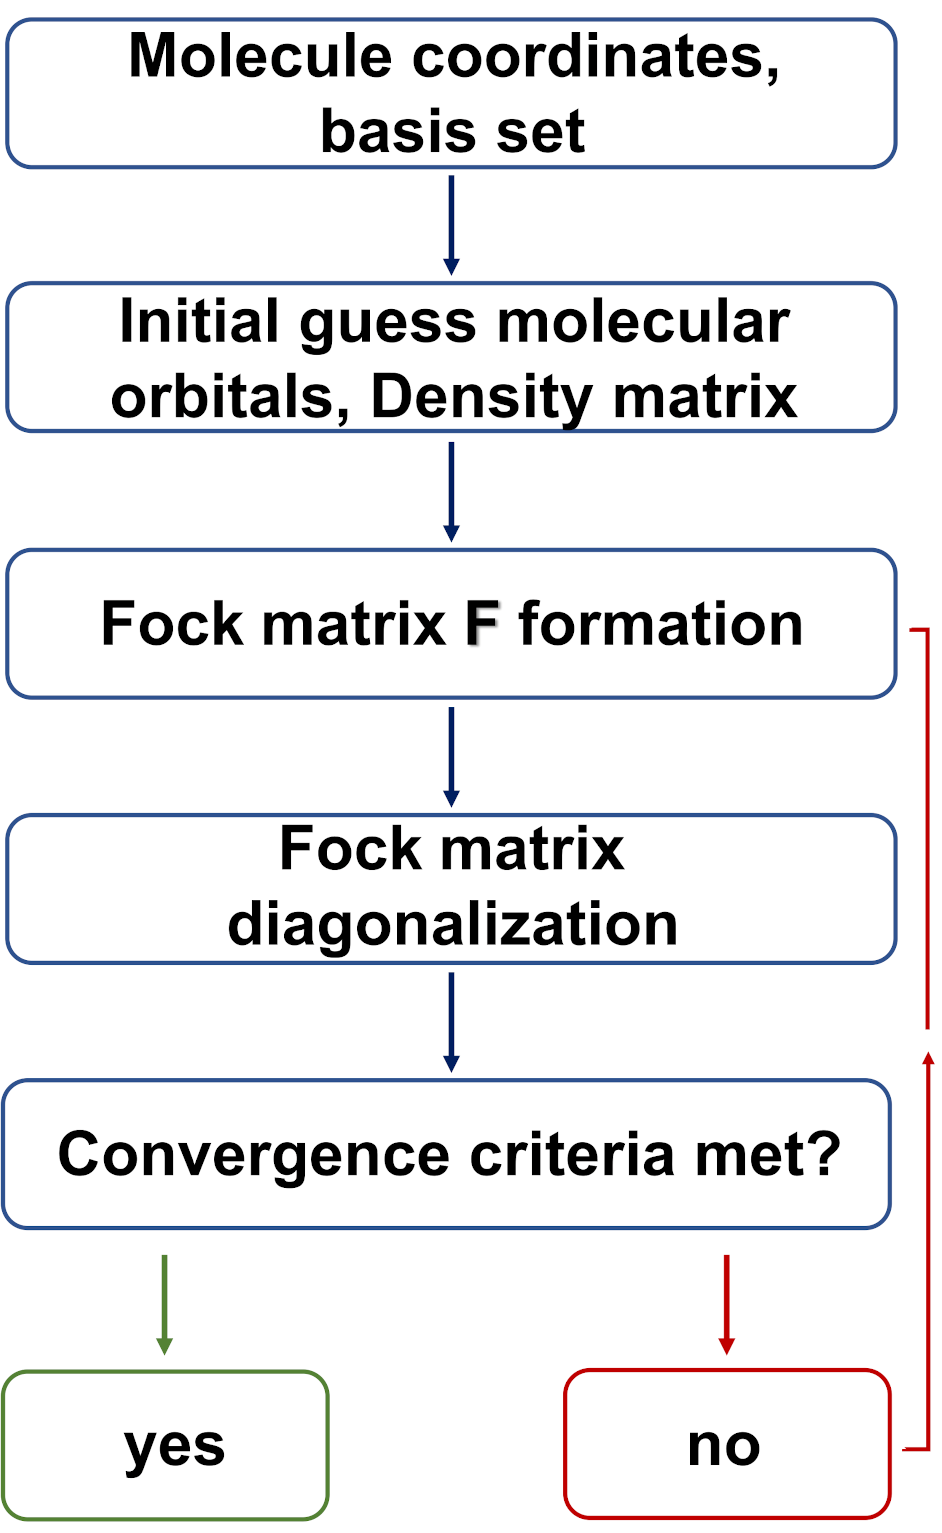
\includegraphics[width=0.4\textwidth]{figures/Flowchart for the HF SCF method.png} 
\caption{Flowchart for the HF SCF method.} \label{HF SCF method}
\end{figure} \\
To write the algorithm efficiently on a computer we can use a matrix formulation. We consider the spatial part of the orbitals as a combination of functions from the basis set $\{ |\phi_{\nu}\rangle \}$,
\begin{equation}
    |\psi({\bf r}_i)\rangle = \sum_{\nu = 1}^K C_{\nu i} |\phi_{\nu}({\bf r}_i)\rangle,
\end{equation}
where $C_{\nu i}$ are real coefficients. \\
Then we can substitute the formula in the HF equation, multiply by $\langle \phi_{\mu}|$, integrate over all space and define two integrals,
\begin{equation}
    S_{\mu \nu} = \int d{\bf r}_i \langle \phi_{\mu}({\bf r}_i)|\phi_{\nu}({\bf r}_i)\rangle,
\end{equation}
called the 'overlap matrix' and
\begin{equation}
    F_{\mu \nu} = \int d{\bf r}_i \langle \phi_{\mu}({\bf r}_i)| f({\bf r}_i) |\phi_{\nu}({\bf r}_i)\rangle,
\end{equation}
called the 'Fock matrix'. \\
The HF equation can be written as
\begin{equation}
    FC = SC\epsilon,
\end{equation}
which is called the 'Roothann equation' \cite{Shikano2021Jun}. Solving the equation means find the square $K\times K$ matrix $C$ that minimizes the system's total energy. \\
This result leads us to write the wave function of our system. \\
\\
Generally, having $N$ electrons and $m>N$ spin-orbitals, we can construct \\
$\left( \begin{array}{c} m \\ N \end{array} \right) = \dfrac{m!}{N!(m-N)!}$ Slater determinants, where a Slater determinant is the antisymmetric combination of the orbitals
\begin{equation}
|\Psi_{HF}({\bf x}_0, ..., {\bf x}_{N-1})\rangle =
\frac1{\sqrt{N!}}
\begin{vmatrix}
    |\chi_{0}({\bf x}_0)\rangle & |\chi_{1}({\bf x}_0)\rangle & ... & |\chi_{m-1}({\bf x}_0)\rangle\\ 
    |\chi_{0}({\bf x}_1)\rangle & |\chi_{1}({\bf x}_1)\rangle & ... & |\chi_{m-1}({\bf x}_1)\rangle\\
    . & . & . & . \\
    . & . & . & . \\
    |\chi_{0}({\bf x}_{N-1})\rangle & |\chi_{1}({\bf x}_{N-1})\rangle & ... & |\chi_{m-1}({\bf x}_{N-1})\rangle
\end{vmatrix}.
\end{equation}
We must combine the spin-orbitals this way in order to be consistent with the Pauli exclusion principle, which states that two fermions can not occupy the same quantum state, i.e. the same orbital. Thus, the probability of that kind of system to be measured must be zero and the wave function must be antisymmetric with respect to particle exchange. \\
However, the Hartree-Fock approach considers only one Slater determinant, called the Hartree-Fock ground state determinant, this is because in the algorithm we only consider the occupied orbitals in order to compute the potential $v^{HF}$. The other determinants represent the excited states of the electronic system. \\
\\
Algorithms like this can be analyzed with respect to their computational cost or requirements. We will define it more precisely in Chapter \ref{Quantum computing for computational chemistry: FTQC devices}, but for now we refer to it as the resources needed to run an algorithm. \\
The computational cost of the Hartree-Fock method scales as $O(m^4)$, due to the calculation of the one- and two-electrons integrals for the mean-field potential, where $m$ is the number of basis functions. \\
This is the lowest cost we will consider in this thesis. \\
\\
The fact that we consider only a single Slater determinant is fundamental, because the HF method, as a mean-field approach, is a strong approximation, which can not give us the exact solution for the system, especially for many-electrons systems where the interaction potential is not negligible. \\
First, electrons in this model do not instantaneously interact with each other, but rather each and every electron interacts with the average field. In reality their movements take into account the positions of all other electrons, in order to avoid being in the same quantum state, i.e. locations in a close proximity. This effect is called 'dynamic correlation' since it is directly related to electron dynamics. This correlation accounts for the short-range structure of the wave function and weak long-range interactions such as London dispersion forces. \\
Secondly, in certain cases an electronic state can be well described only by a linear combination of more than one Slater determinant, this is obvious since, as we said before, wave functions are not localized and electrons can be found in different locations, i.e. different orbitals. This is called 'static correlation' and is associated with the strong mixing of degenerate or near-degenerate determinants. \\
More properly we say that the total energy of the system is
\begin{equation}
    E_{exact} = E_{HF} + E_{correlation},
\end{equation}
so we still need to take into account the correlation term, which derives from the electrons interaction. \\
This is why in the decades following the definition of the HF method, scientists came up with new methods to tackle these problems. These go under the name of post-HF methods. \\
\\
The most intuitive one is the 'configuration interaction' (CI) method. 'Configuration' means that we write the wave function as a linear combination of Slater determinants and 'interaction' means that we mix different electronic states in order to account for electronic correlation. The first term in the expansion is normally the Hartree–Fock determinant and the subsequent ones are the states in which one spin-orbital at a time is swapped with a virtual orbital. If only one spin-orbital differs, we describe this as a single excitation determinant (CIS). If two spin-orbitals differ it is a double excitation determinant (CID) and so on. This is used to limit the number of determinants in the expansion which is called the CI-space. If the expansion includes all possible state functions it is called a 'full configuration interaction' (FCI) method,
\begin{equation}
    |\Psi_{FCI}\rangle = (I + \sum_{i,\alpha} C_{i\alpha} a^\dagger_i a_\alpha
                        + \sum_{i>j,\alpha>\beta} C_{ij\alpha\beta} a^\dagger_i a^\dagger_j a_\alpha a_\beta
                        + ...) |\Psi_{HF}\rangle,
\end{equation}
where $a^\dagger_i$ and $a_\alpha$ are the creation and destruction operators used to swap the spin-orbitals, i.e., in the second quantization scheme, destroy a fermion in the occupied state $\alpha$ and create one in the virtual state $i$. $C$ are parameters to be optimized according to the Rayleigh-Ritz variational principle, which states that the energy expectation value of a parametrized wave function is greater than or equal to the lowest energy eigenvalue of the Hamiltonian being measured. \\
The FCI exactly solves the electronic TISE, because it takes into account all the Slater determinants \cite{Cao2019Oct}. This also means that the computational cost to execute this algorithm grows combinatorially, because for each new orbital we have to consider all the possible ways the electrons occupy the orbitals. Thus the computational cost of the FCI method is $O(m!)$, which is the highest scaling we can consider. \\
All the others computational methods aim to find the same results while being less expensive in the scaling of the resources, this leads to a trade-off between accuracy and computational requirements. As a standard to frame these methods we will refer to the 'chemical accuracy', which is defined as an error of 1 kcal/mol, or equivalently 4 kJ/mol or 1 mHa, with resepect to the hypothetical exact energy or an error present in an experimental measurement to find thermodynamic properties. This is the target for every simulation to be comparable with real data. \\
\\
An important post-HF method is the Møller–Plesset (MP) perturbation theory. \\
The idea is to take advantage of Rayleigh–Schrödinger perturbation theory. We write the Hamiltonian as
\begin{equation}
    H = H_0 + \lambda V,
\end{equation}
with
\begin{equation}
    H_0 = \sum_i f({\bf x}_i).
\end{equation}
We can expand the ground state eigenfunction and eigenvalue as a Taylor series in $\lambda$:
\begin{equation}
    |\Psi_0\rangle = |\Psi_{0}^{(0)}\rangle + \lambda|\Psi_{0}^{(1)}\rangle + \lambda^2|\Psi_{0}^{(2)}\rangle + ... \ , \label{perturbation}
\end{equation}
\begin{equation}
    E_0 = E_0^{(0)} + E_0^{(1)} + E_0^{(2)} + ... \ ,
\end{equation}
where $|\Psi_{0}^{(0)}\rangle = |\Psi_{HF}\rangle $ and $E_0^{(0)} = E_{HF}$. \\
By imposing the normalization of the wave function and by solving the equation (\ref{perturbation}) iteratively for each power of the expansion, we obtain the corrections for the ground state eigenfunction and eigenvalue. For example
\begin{equation}
    E_0^{(1)} = \langle\Psi_{0}^{(0)}|V|\Psi_{0}^{(0)}\rangle,
\end{equation}
\begin{equation}
    E_0^{(2)} = \sum_{j>0} \frac{|\langle\Psi_j^{(0)}|V|\Psi_{0}^{(0)}\rangle|^2}{E_0^{(0)} - E_j^{(0)}}
\end{equation}
and so on. \\
One usually truncates the expansion due to its computational cost and the resulting methods are called MP2, MP3, etc., where the number indicate the order of the expansion. \\
\\
The last method we analyze is the 'coupled cluster' (CC) method. Just like the CI method, the goal is to add terms to the Hartree-Fock wave function to account for correlation. \\
The expansion is written as
\begin{equation}
    |\Psi_{CC}\rangle = \prod_{i,\alpha} (I + C_{i\alpha} a^\dagger_i a_\alpha)
                        \prod_{i>j,\alpha>\beta} (I + C_{ij\alpha\beta} a^\dagger_i a^\dagger_j a_\alpha a_\beta) ... |\Psi_{HF}\rangle
\end{equation}
and it can be reformulated as
\begin{equation}
    |\Psi_{CC}\rangle = e^T |\Psi_{HF}\rangle,
\end{equation}
where
\begin{equation}
    T = T_1 + T_2 + ... = \sum_{i,\alpha} t_{i\alpha} a^\dagger_i a_\alpha + \frac14 \sum_{i>j,\alpha>\beta} t_{ij\alpha\beta} a^\dagger_i a^\dagger_j a_\alpha a_\beta + ...
\end{equation}
Again we swap spin-orbitals to build more Slater determinants other than than the HF one. $\alpha$ and $\beta$ indicate occupied orbitals, $i$ and $j$ indicate virtual orbitals and $t$ indicates excitation amplitudes. \\
When all of the excitation operators $T_i$ are included, the CC method recovers the FCI wave function and again this calculation is very costly, so the method is normally truncated to a lower excitation level, often single (CCS) and double excitations (CCSD). \\
Because of its product parametrization, the CC method generates a trial wave function that includes all possible powers of $T_i$ operators, this way it provides faster convergence than the CI method. \\
The CC method is often referred to as the "gold standard" for chemistry simulation. \\
The CCSD(T) method, where the T inside the brackets means it is calculated only perturbatively, is known to treat dynamic correlation accurately, but is generally inapplicable to molecular problems dominated by non-dynamic correlation \cite{Elfving2020Sep}. \\
\\
All these methods can be analyzed and compared with respect to the total scaling, i.e. the computational cost. The result we have is \cite{BibEntry2006Aug}
\begin{equation}
\begin{matrix}
    HF \approx DFT & < & MP2 & < & CISD \approx CCSD & < & MP4 \approx CCSD(T) & << & FCI \\
    O(m^{3-4}) & < & O(m^5) & < & O(m^6) & < & O(m^7) & << & O(m!) \label{classical scaling}
\end{matrix}
\end{equation}
where DFT means density functional theory, which is described in Chapter \ref{Density functional theory}. \\
At first glance we can easily notice that the cost scales up very quickly even though the methods are inaccurate, since they approximate the FCI wave function. This is one of the reasons that makes us look towards a full quantum approach.

\subsection{Accuracy and precision}
The most useful measure of accuracy for applications involving chemical reactions is chemical accuracy, defined before. This is a desirable target because calculations capable of achieving it would rival the accuracy of measurements attainable in a chemical laboratory. \\
However, it is important to distinguish accuracy (computational error with respect to an experimental measurement) from precision (computational error with respect to a computational reference, for example, a sufficiently accurate result obtained with a large basis set). A simplified representation is shown in Figure \ref{Accuracy vs precision}.
\begin{figure}[ht]
\centering
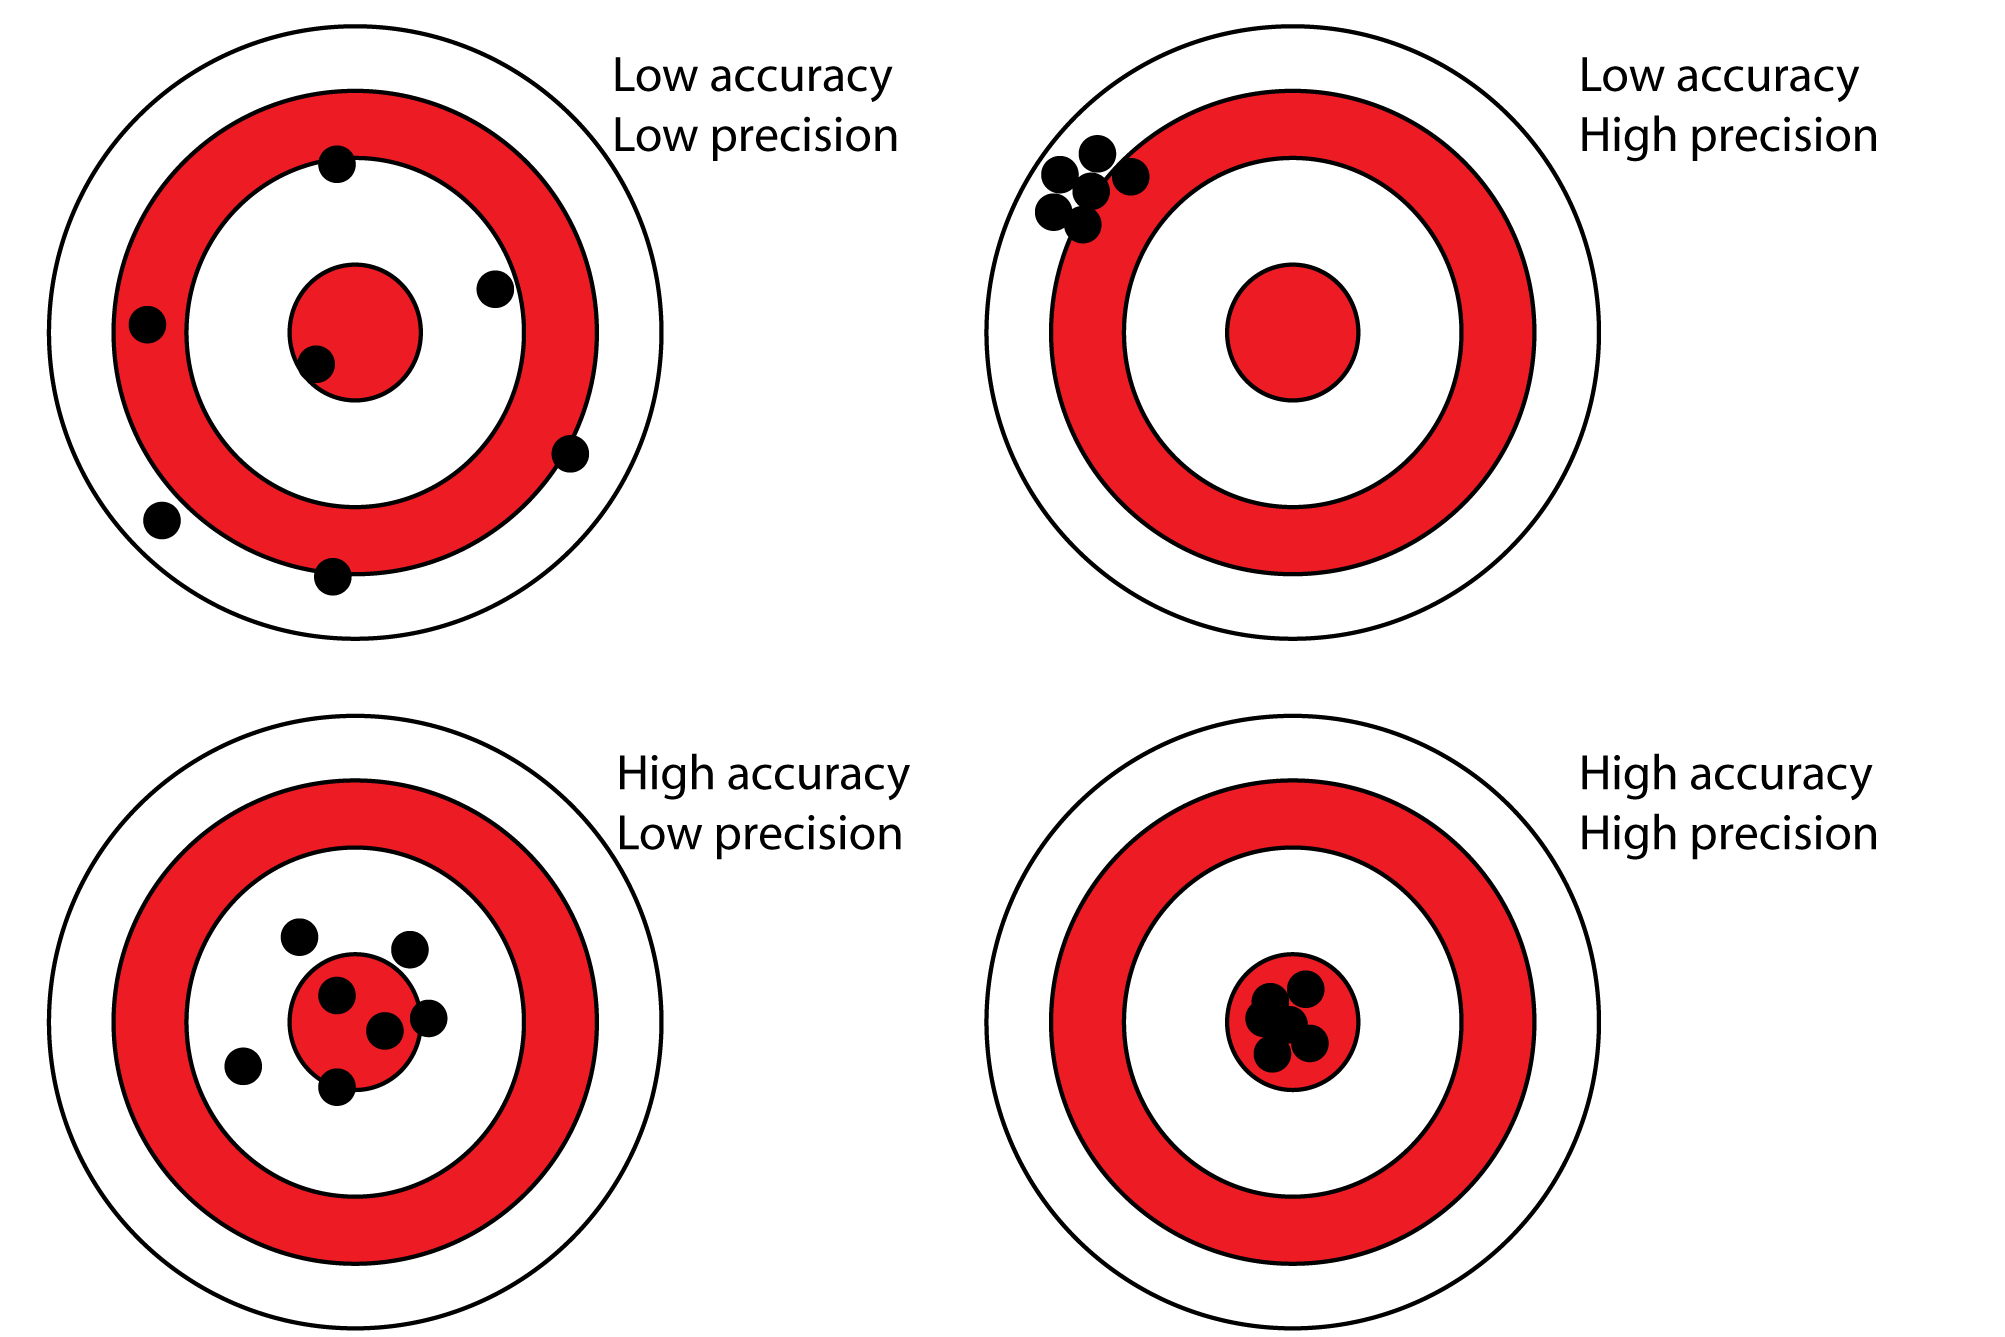
\includegraphics[width=0.7\textwidth]{figures/Accuracy vs precision.jpg}
\caption{Accuracy vs precision.} \label{Accuracy vs precision}
\end{figure} \\
Several studies described experiments that reached chemical accuracy, but in reality they reached chemical precision: an error of at most 1 kcal/mol compared to the exact solution typically provided by the combination of the FCI method and a very small basis set that was used as a reference. \\
This is an important distinction because an answer computed with a 1 kcal/mol precision may be useless for explaining or predicting chemical reactivity if the level of theory used as a reference does not allow a similar level of accuracy. Matching an FCI energy value is not necessarily a practically useful achievement, it means attaining a good precision but not a high accuracy. \\
Configuration interaction (including FCI) energies obtained with Gaussian basis sets converge to the "exact" energy very slowly. Therefore one needs Gaussian basis sets of at least quadruple-$\zeta$ quality (where $\zeta$ is the number of contracted functions per atomic orbital) to achieve chemical accuracy with pure, non-extrapolated FCI calculations.

\section{Quantum approach}
As mentioned in the introduction, in 1982 Richard Feynman gave a speech titled "Simulating Physics with Computers" at the California Institute of Technology, where he stated \cite{Feynman1982Jun}:
\begin{displayquote}
    \textit{"And I'm not happy with all the analyzes that go with just the classical theory, because nature isn't classical, dammit, and if you want to make a simulation of nature, you'd better make it quantum mechanical, and by golly it's a wonderful problem, because it doesn't look so easy."}
\end{displayquote}
This thought was the beginning of a massive research for the 'exact method' and the 'perfect computer' to perform the simulation of an atomic system. \\
\\
The problem with classical computation is that if one wants to perfectly simulate a quantum system, the calculation must take into account all the possible states in which the wave function can be found, this can be made via encoding and evaluation of the wave function on a discretized spatial grid in the position representation $\{ {\bf r} \} $ or on a basis set in the orbitals representation. In both cases one can see that the representation, and therefore the memory to store the representation, grows superpolinomially as the system (i.e. the number of electrons and the number of configurations) grows. \\
\\
In the grid-based method a wave function can be written as
\begin{equation}
    |\Psi\rangle = \sum_{{\bf x}_1,...,{\bf x}_N} \psi({\bf x}_1,...,{\bf x}_N) \mathcal{A} (|{\bf x}_1,...,{\bf x}_N\rangle)
\end{equation}
where $|{\bf x}_i\rangle = |{\bf r}_i\rangle |\sigma_i\rangle$ is a spatial and spin coordinate, $|{\bf r}_i\rangle = |x_i\rangle |y_i\rangle |z_i\rangle, \ \forall i \in \{1,2,...,N\}, \ x_i,y_i,z_i \in \{0,1,...,P-1\},$ and $\sigma_i \in \{0,1\}$. In total there are $P^{3N} \times 2^N$ complex amplitudes $\psi$ to store, thus the the memory required scales exponentially with the size of the simulated system. \\
\\
In the basis set method (let's take the second quantization scheme for simplicity) to write down a Slater determinant we only need to indicate which spin-orbitals are occupied by electrons
\begin{equation}
    |\Psi\rangle = |n_0,n_1,...,n_i,...,n_{m-1}\rangle,
\end{equation}
where $|n_i\rangle$ is the occupation number and it indicates the number of particles in spin-orbital $|\chi_i\rangle$, thus $|n_i\rangle = 1$ when $|\chi_i\rangle$ is occupied and $|n_i\rangle = 0$ when $|\chi_i\rangle$ is unoccupied, these are the only two possible values since we are working with fermions that follow Pauli exclusion principle, if we worked with bosons $|n_i\rangle$ would take values from 0 to $\infty$. It is implied that the vector of occupation numbers has to be antisymmetrized and normalized when we expand it, e.g.
\begin{equation}
    |1,1,0,...,0\rangle = \frac{1}{\sqrt{2}} (|\chi_1({\bf x}_1)\rangle |\chi_2({\bf x}_2)\rangle - |\chi_2({\bf x}_1)\rangle |\chi_1({\bf x}_1)\rangle).
\end{equation}
Hence one can see that, as the number of electrons grows, the number of configurations grows combinatorially as $\binom{m}{N}$, as we have seen before for the FCI wave function, and the memory scales in the same way. \\
\\
One can also consider the most simple and fundamental encoding in the computational basis, let's say that a system, e.g. a particle, can be found in states $|0\rangle$, ground state, or $|1\rangle$, excited state, the generic wave function for this two-state system is
\begin{equation}
    |\Psi\rangle = \gamma_0 |0\rangle + \gamma_1 |1\rangle,
\end{equation}
due to superposition. If we now add a new particle and write down the wave function for the composite system this becomes
\begin{equation}
    |\Psi\rangle = \gamma_{00} |00\rangle + \gamma_{01} |01\rangle + \gamma_{10} |10\rangle + \gamma_{11} |11\rangle,
\end{equation}
this is because in quantum mechanics states are vectors of Hilbert spaces and when we describe composite systems we have to take the tensor product of all the basis states of the Hilbert spaces of the individual systems. One can easily see that, adding more and more particles to this simple system, the number of states grows exponentially as $2^N$, where $N$ is the number of particles in the composite system, and so grows the memory required to store all of these states. \\
This argument focuses only on the computational memory to store the wave function, i.e. all the information necessary to describe a quantum system, let alone the requirements to simulate the evolution of such wave function. In general one has to store the complete Hamiltonian, which, in a descrete finite space, is a matrix with the same size of its eigenvectors, i.e. the states of the wave function. Thus if the wave function needs $2^N$ complex numbers to be stored, the Hamiltonian needs $2^N \times 2^N$ complex numbers, which is an extraordinary amount of resources. For example, a 40 spin-$\frac12$ particles need $2^{40} \approx 10^{12}$ numbers and its Hamiltonian needs a $2^{40} \times 2^{40}$ matrix with $\approx 10^{24}$ entries. \\
\\
In this context Feynman's idea is simple: if we want to study a physical system (P), is it possible to take a simulator system (S) which resembles system P, elaborate it via the laws of quantum mechanics, extract properties and then translate them back to system P? \\
If the system S follows the laws of quantum mechanics than the encoding of the wave function and its evolution will translate naturally from one system to the other.
\begin{figure}[ht]
\centering
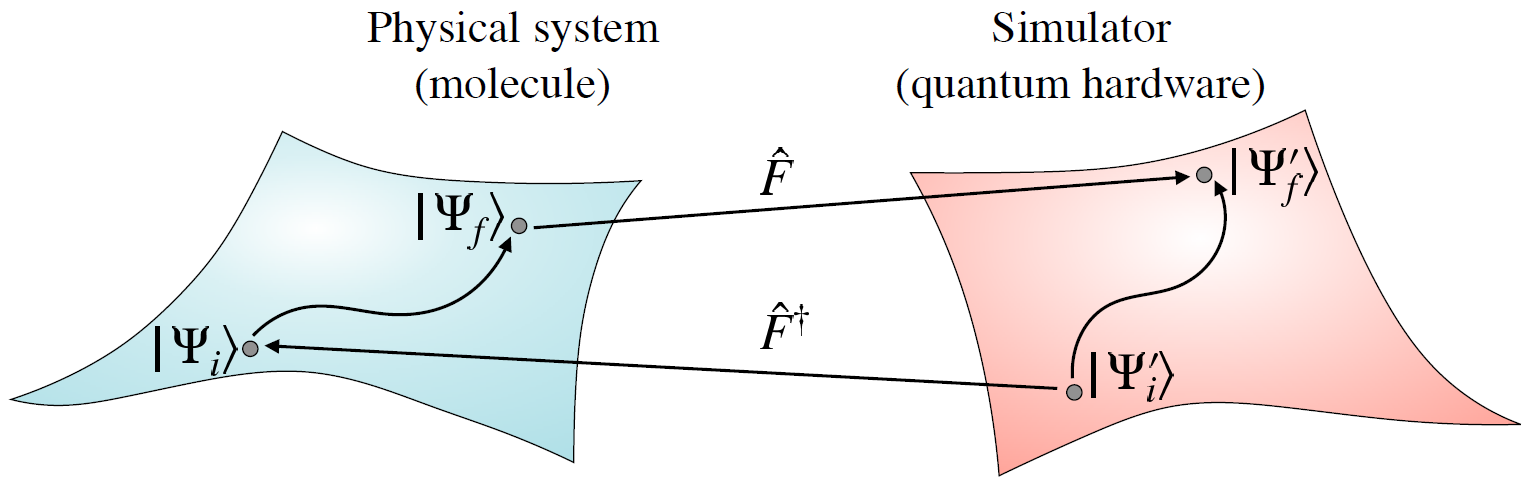
\includegraphics[width=0.95\textwidth]{figures/Simulation.png}
\caption{Scheme for the simulation of a physical system \cite{Motta2021Dec}.}
\end{figure} \\
The system S is the one we can manipulate, this is what is called a 'universal quantum computer'. In the years next to Feynman's speech many researchers refined this intuition. First of all how is this simulator made, i.e. what kind of hardware one needs? And then what type of manipulations one needs to do, i.e. what kind of software or algorithm? \\
The history of quantum computers is full of new discoveries year by year, among the most admirable are Shor's algorithm, for finding the prime factors of an integer \cite{Shor1994Nov}, and Grover's algorithm, for unstructured search \cite{Grover1996Jul}, but we will only focus on the simulation of atomic systems. \\
In 1996 Seth Lloyd \cite{Lloyd1996Aug} found out a way to carry on a simulation 'efficiently' (in Chapter \ref{Quantum computing} we will give a definition of what efficiently means), he used qubits, which are the most simple two-state systems, in analogy to classical bits, to naturally store all the information about the wave function, and demonstrated that if the physical systems evolve according to local interactions, i.e. $H = \sum_i h_i$, their evolution can be written using the Lie-Trotter-Suzuki decomposition, commonly referred to as Trotterization,
\begin{equation}
    U = e^{-iHt} = e^{-i\sum_i h_i t} = \left( \prod_i e^{-i h_i t/S} \right)^S + O(t^2 / S),
\end{equation}
where each operator can be applied $S$ times to regain the full time evolution. \\
Similarly in 2005 Alan Aspuru-Guzik et al. \cite{Aspuru-Guzik2005Sep} described an algorithm to provide a solution for eq. (\ref{eq:electronic TISE}), i.e. find the energy of the ground and the excited states of a system. The algorithm exponentiates the eigenvalues of the Hamiltonian and retrieve them through the quantum Fourier transform (QFT), a version of the Fourier transform designed for quantum computers. \\
These two algorithms go under the name of quantum phase estimation (QPE) algorithms, since the goal of them is to find the phase of the exponential in the evolution formula, in this case the energy of the system. \\
Remaining in the field of quantum computation applied to chemical simulations, in 2014 Alberto Peruzzo et al. \cite{Peruzzo2014Jul} derived another algorithm called variational quantum eigensolver (VQE). This is a hybrid quantum-classical algorithm since, after the manipulation, the measured values are optimized iteratively through a classical computer, as it happens in machine learning algorithms. This algorithm was meant to be run on a quantum computer with low computing power, the so-called noisy intermediate-scale quantum (NISQ) devices, which we describe in Chapter \ref{Quantum computing for computational chemistry: NISQ devices}, in stark contrast to previous algorithms which were meant to be run on a quantum computer with high computing power, the so-called fault-tolerant quantum computation (FTQC) devices, which we describe in Chapter \ref{Quantum computing for computational chemistry: FTQC devices}.